\documentclass{standalone}
\usepackage{xcolor,amsmath,amssymb,amsfonts}
\usepackage{fontspec}
\usepackage[T1]{fontenc}
\usepackage[tt=false, type1=true]{libertine}
\usepackage[libertine]{newtxmath}

\usepackage{tikz}
\usetikzlibrary{arrows.meta}
\definecolor{red}{HTML}{c63a44}
\begin{document}

$$
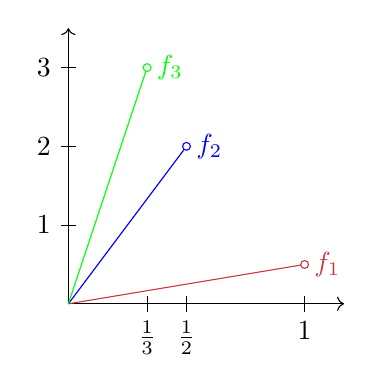
\begin{tikzpicture}
    \draw[->] (0, 0) -- (0, 3.5);
    \draw (0.1, 1) -- (-0.1, 1) node [anchor=east, align=right] {1};
    \draw (0.1, 2) -- (-0.1, 2) node [anchor=east, align=right] {2};
    \draw (0.1, 3) -- (-0.1, 3) node [anchor=east, align=right] {3};
    \draw[->] (0, 0) -- (3.5, 0); 
    \draw (1.5, 0.1) -- (1.5, -0.1) node [anchor=north, align=center] {$\frac12$};
    \draw (3, 0.1) -- (3, -0.1) node [anchor=north, align=center] {1};
    \draw (1, 0.1) -- (1, -0.1) node [anchor=north, align=center] {$\frac13$};
    \draw[red] (0, 0) -- (3, 0.5) node [anchor=west] {$f_1$};
    \node[red, circle, draw=red, inner sep=1, fill=white] at (3, 0.5) {};
    \draw[blue] (0, 0) -- (1.5, 2) node [anchor=west] {$f_2$};
    \node[blue, circle, draw=blue, inner sep=1, fill=white] at (1.5, 2) {};
    \draw[green] (0, 0) -- (1, 3) node [anchor=west] {$f_3$};
    \node[green, circle, draw=green, inner sep=1, fill=white] at (1, 3) {};    
\end{tikzpicture}
$$

\end{document}